\documentclass[11pt,a4paper]{report}
\usepackage[latin1]{inputenc}
\usepackage{amsmath}
\usepackage{amsfonts}
\usepackage{amssymb}
\usepackage{verbatim}
\usepackage[usenames]{xcolor}
\usepackage{graphicx}
\usepackage{hyperref}
\usepackage{cite}
\usepackage[margin=0.9in]{geometry}
\author{Jeremy Moss}

\begin{document}
	
	\begin{center}
	\section*{Developing a photometric estimate of quasar redshifts}
	\subsection*{An independent measure to the distances to\\the most powerful objects in the Universe}
	\end{center}
	
%	\begin{flushright}
%	Jeremy Moss	
%	\end{flushright}

	\subsubsection*{Motivation}
	Hydrogen is the most common form of baryonic (normal) matter, and is the
	fundamental building block of all stars, which subsequently provide the heavier elements
	found in planets and life. As such, it plays a critical role in our
	understanding of the history and evolution of our Universe. Hydrogen emits radio
	waves with a characteristic wavelength of 21 cm. Unlike visible light, radio
	waves are not absorbed or scattered by interstellar dust, water vapour and
	daylight, being observable from Earth 24 hours a day, and across the entire
	Universe.\\
	
	To search for an object in any wavelength, we need to know not only its	position in the sky, but also a redshift to which to tune the receiver. This
	redshift is related closely to the distance to the object (see
	Figure~\ref{fig:absorber}), and usually, this comes from spectroscopic observation of
	its optical light. Since intervening clouds of dust and gas absorb visible light, this introduces a selection bias against dimmer sources, those which contain the cold, neutral gas. Optically dim objects which are
	rich in hydrogen remain undetected, even with the world's largest optical
	instruments; thus, being able to determine the redshift without requiring an optical spectrum would be extremely useful.\\\\
	
	\begin{figure}[h!]
		\centering
		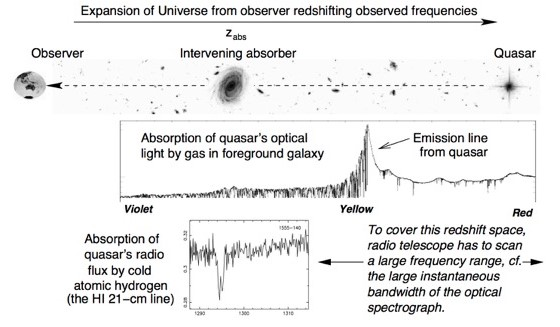
\includegraphics[scale=1.2]{absorber.jpeg}
		\caption[21 cm radiation is absorbed by the cool gas in an intervening
		object]{{\small The radiation from a quasar is absorbed at a (rest-frame) wavelength of
			21 centimetres by the cool hydrogen gas in an intervening galaxy or cold gas cloud.}}
		\label{fig:absorber}
	\end{figure}
	
	Most large galaxies contain a supermassive black hole (SMBH), nestled at the
	core of the galaxy. This black hole can mass in the range of millions, to
	billions of solar masses. For example, our Milky Way Galaxy's black hole has a
	mass of approximately 4.2 million solar masses \cite{bland}. With such a relatively small mass, our galactic black hole is inactive.
	In galaxies with an extremely large SMBH, the surrounding accretion disk can give off huge amounts of energy in ultraviolet radiation, in some cases on the order of
	10$^{39}$ watts \cite{2013ApJ...762...49B}. This is called an \textit{active galactic nucleus} (AGN), or
	\textit{quasar}. This phenomenal energy output allows quasars to be visible across the entire Universe.\\
	
	In the case of some of the most active of AGNs, such as
	\href{https://en.wikipedia.org/wiki/S5_0014\%2B81}{S5~0014+81}, the central
	black hole is accreting material at a rate of several Earth-masses per second
	(\href{http://www.astro.keele.ac.uk/~rdj/}{Prof. Rob Jeffries},
	\href{https://www.keele.ac.uk/}{University of Keele, Staffordshire, UK}
	[personal communication, July 4, 2018]). Figure~\ref{fig:3C273} shows another example; 3C273, the first quasar identified. 
	\\
	
	\begin{figure}[h!]
		\centering
		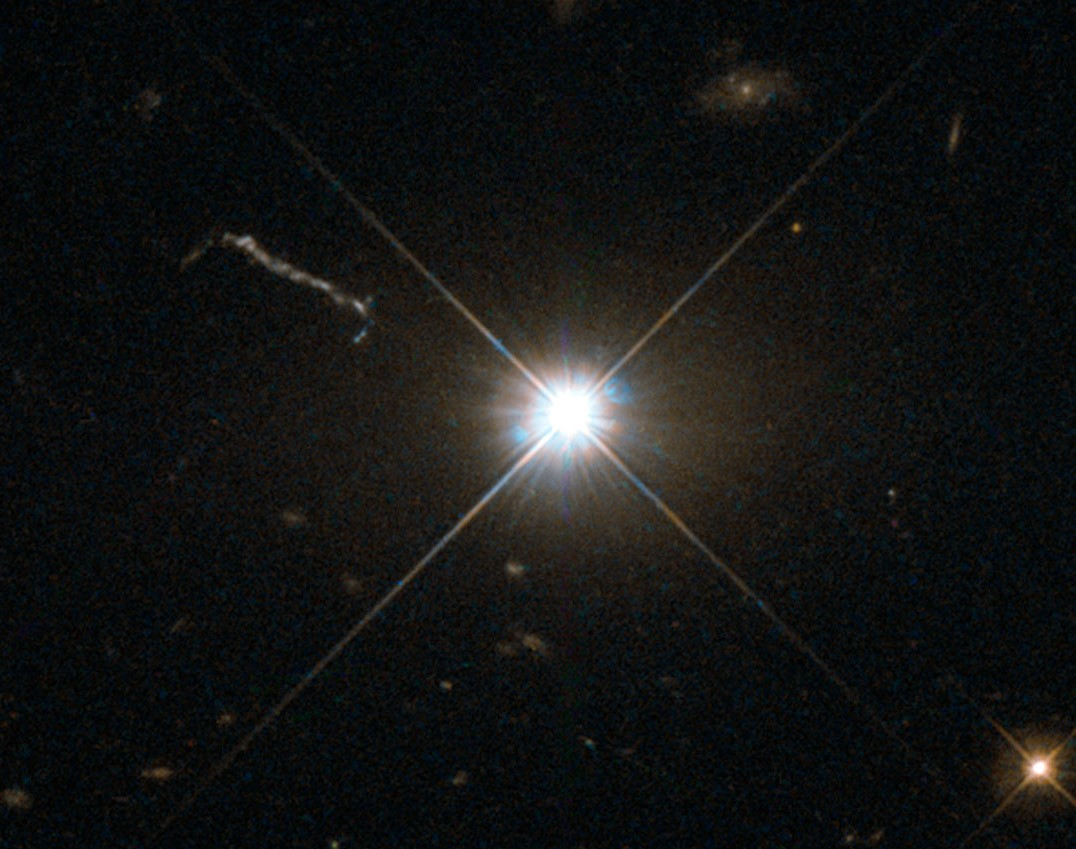
\includegraphics[scale=0.2]{3C273.jpg}
		\caption[3C273, one of the brightest known quasars]{{\small One of the brightest known
				quasars, and, in 1963, the first ever discovered,  \href{https://www.spacetelescope.org/images/potw1346a/}{3C273}, is
				accreting roughly 0.2 Earth masses per second. Note the presence of a
				\href{https://ned.ipac.caltech.edu/level5/March02/Courvoisier/Cour6.html}{jet}
				of charged particles (10~o'clock position) propelled outward by the energy
				generated near the black hole. This jet measures some 200,000 light-years in
				length.}}
		\label{fig:3C273}
	\end{figure}
	
	

	\subsubsection*{Project description}
	
	A correlation has been found between the near-infrared \textit{K}-magnitude ($\lambda = 2.2 \mu$m) and the redshift of the source \cite{glowacki}. See Figure \ref{fig:galaxy_fit}.
	The WISE spacecraft (\textit{Wide-field Infrared Survey Explorer}) makes observations in four mid-infrared wavelength range bands: 3.4, 4.6, 12 and 22 $\mu$m. The correlation is also apparent at the \textit{W1} band ($\lambda
	= 3.4 \mu$m), since these two wavelengths are reasonably close. This means that the redshifts of galaxies with relatively quiescent central black holes can be reasonably predicted from their apparent near-infrared flux. Some correlation is to expected, since objects which are farther away are fainter, but the fact that it is so linear is remarkable. We would expect each galaxy to have its own individual properties, but the tight linear correlation suggests that these properties have little influence on the magnitude.\\
	
	However, when the same method is applied to quasars, we find that
	the \textit{K-z} fit drastically underestimates the redshift of the source (Figure \ref{fig:quasar_fit}).
	This is probably because, in the case of a quasar, the light spectrum is dominated by the
	AGN, in addition to the galactic stellar population. This results in a higher
	emission in the near infra-red wavelengths than the galactic model predicts.\\
	

	\begin{figure}[h!]
		\centering
		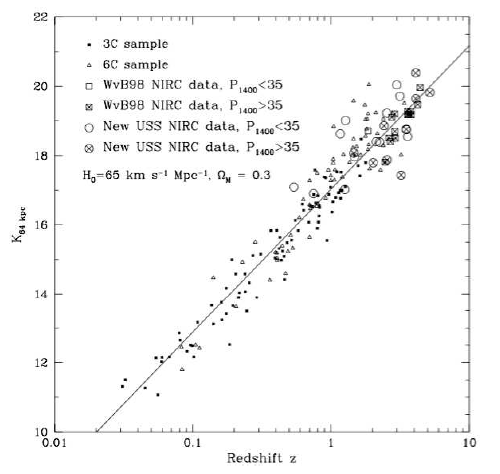
\includegraphics[scale=0.85]{galaxies_fit.PNG}
		\caption[Fit for galaxies]{{\small Plot of \textit{K}-magnitude ($\lambda
			= 2.2 \mu$m) against redshift for galaxies. Such a tight fit is remarkable, since each galaxy has its own individual properties. \textit{K}-magnitude is $K = 4.43\log_{10}z + 17$}}
		\label{fig:galaxy_fit}
	\end{figure}

	\begin{figure}[h!]
		\centering
		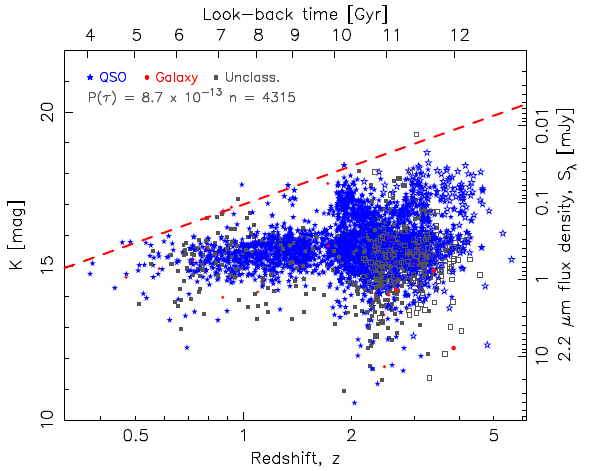
\includegraphics[scale=0.8]{quasars_fit.PNG}
		\caption[Fit for quasars]{{\small Plot of \textit{K-z} fit for a large sample of quasars. The broken line shows the above fit for galaxies, demonstrating that the \textit{K}-magnitude underestimates redshift in the case of quasars.}}
		\label{fig:quasar_fit}
	\end{figure}
	\newpage
		This work will benefit some of the world's largest multi-wavelength surveys,
	including the
	\href{https://en.wikipedia.org/wiki/Square_Kilometre_Array}{\textit{Square
			Kilometre Array}} (SKA) and its pathfinder \textit{Australian SKA Pathfinder} (\href{https://en.wikipedia.org/wiki/Australian_Square_Kilometre_Array_Pathfinder}{ASKAP}). For example, the \textit{Evolutionary Map of the
		Universe} (EMU) \cite{2011PASA...28..215N}, a survey on the ASKAP, will detect about 70 million radio
	sources, and most of these will be galaxies containing massive black holes. Due
	to the nature of the survey, the spectra taken by EMU will be of insufficient
	resolution to determine the redshifts. If these can be estimated from the
	photometry, the value of the survey in determining how gas, stars and energetic
	phenomena such as black holes and quasars are distributed throughout the
	Universe will increase dramatically. Even an approximate or statistical estimate of the redshift would be valuable.\\
	
%	\newpage
	\subsubsection*{Aim}
	These observations show strong correlations between the
	\textit{K}-magnitude and \textit{z} for quasars \cite{2018MNRAS.476.3580C}
	, giving a straight-line fit in $\log$-space, but
	the regression coefficient is too low (\textit{i.e.} the points are too
	scattered) to provide a useful estimate of the redshift of the object.\\
	
	This project aims to find a magnitude, or a combination of magnitudes, which
	can improve the prediction of the straight-line fit to quasar sources by
	maximising the regression coefficient to account for the contribution in near
	infra-red wavelengths of the AGN. In this way, we aim to find a relation close
	enough to make redshift predictions. If successful, this work will also give
	great insight into the contribution of the black hole to the photometry of these
	objects, leading to an improved understanding of the underlying physical
	processes in the most powerful objects in the Universe.
	
	
	\bibliography{bibliography_file}
	\bibliographystyle{plain}

	
\end{document}
